%{{第七十八回}}{第七十八回}}

\chapter{老学士闲征姽婳词\hspace{.5em}痴公子杜撰芙蓉诔}
{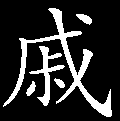
\includegraphics[width=3mm]{../Images/00005}\kaishu 文有宾主,不可误。此文以《芙蓉诔》为主,以《}姽婳{\kaishu 词》为宾,以宝玉古歌为主,以贾环贾兰诗绝为宾。文有宾中宾,不可误。以清客作序为宾,以宝玉出游作诗为宾中宾。由虚入实,可歌可咏。}

话说两个尼姑领了芳官等去后,王夫人便往贾母处来省晨,见贾母喜欢,便趁便回道:``宝玉屋里有个晴雯,那个丫头也大了,而且一年之间,病不离身;我常见他比别人分外淘气,也懒;前日又病倒了十几天,叫大夫瞧,说是女儿痨,所以我就赶着叫他下去了。若养好了也不用叫他进来,就赏他家配人去也罢了。再那几个学戏的女孩子,我也作主放出去了。一则他们都会戏,口里没轻没重,只会混说,女孩儿们听了如何使得?二则他们既唱了会子戏,白放了他们,也是应该的。况丫头们也太多,若说不够使,再挑上几个来也是一样。''贾母听了,点头道:``这倒是正理,我也正想着如此呢。但晴雯那丫头我看他甚好,怎么就这样起来。我的意思,这些丫头的模样、爽利、言谈、针线多不及他,将来只他还可以给宝玉使唤得。谁知变了。''

王夫人笑道:``老太太挑中的人原不错。只怕他命里没造化,所以得了这个病。俗语又说:`女大十八变。'况且有本事的人,未免就有些调歪。老太太还有什么不曾经验过的。三年前我也就留心这件事。先只取中了他,我便留心。冷眼看去,他色色虽比人强,只是不大沉重。若说沉重知大礼,莫若袭人第一。虽说贤妻美妾,然也要性情和顺、举止沉重的更好些。就是袭人模样虽比晴雯略次一等,然放在房里,也算得一二等的了。况且行事大方,心地老实,这几年来,从未逢着宝玉淘气。凡宝玉十分胡闹的事,他只有死劝的。因此品择了二年,一点不错了,我就悄悄的把他丫头的月分钱止住,我的月分银子里批出二两银子来给他。不过使他自己知道,越发小心效好之意。且不明说者,一则宝玉年纪尚小,老爷知道了又恐说耽误了书;二则宝玉再自为已是跟前的人不敢劝他说他,反倒纵性起来。所以直到今日才回明老太太。''

贾母听了,笑道:``原来这样,如此更好了。袭人本来从小儿不言不语,我只说他是没嘴的葫芦。既是你深知,岂有大错误的。而且你这不明说与宝玉的主意更好。且大家别提这事,只是心里知道罢了。我深知宝玉将来也是个不听妻妾劝的。我也解不过来,也从未见过这样的孩子。别的淘气都是应该的,只他这种和丫头们好却是难懂。我为此也耽心,每每的冷眼查看他。\elegantpar{只和丫头们闹,必是人大心大,知道男女的事了,所以爱亲近他们。既细细查试,究竟不是为此。岂不奇怪。想必原是个丫头错投了胎不成。}{投错了}''说着,大家笑了。王夫人又回今日贾政如何夸奖,又如何带他们逛去,贾母听了,更加喜悦。

一时,只见迎春妆扮了前来告辞过去。凤姐也来省晨,伺候过早饭,又说笑了一回。贾母歇晌后,王夫人便唤了凤姐,问他丸药可曾配来。凤姐儿道:``还不曾呢,如今还是吃汤药。太太只管放心,我已大好了。''{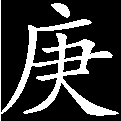
\includegraphics[width=3mm]{../Images/00004}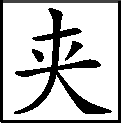
\includegraphics[width=3mm]{../Images/00012}\footnotesize \kaishu 总是勉强。}王夫人见他精神复初,也就信了。{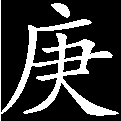
\includegraphics[width=3mm]{../Images/00004}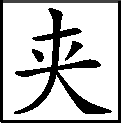
\includegraphics[width=3mm]{../Images/00012}\footnotesize \kaishu 只用此一句,便入后文。}因告诉撵逐晴雯等事,又说:``怎么宝丫头私自回家睡了,你们都不知道?我前儿顺路都查了一查。谁知兰小子这一个新进来的奶子也十分的妖乔,我也不喜欢他。我也说与你嫂子了,好不好叫他各自去罢。况且兰小子也大了,用不着奶子了。我因问你大嫂子:`宝丫头出去难道你也不知道不成?'他说是告诉了他的,不过住两三日,等你姨妈好了就进来。姨妈究竟没甚大病,不过还是咳嗽腰疼,年年是如此的。他这去必有原故,敢是有人得罪了他不成?那孩子心重,亲戚们住一场,别得罪了人,反不好了。''凤姐笑道:``谁可好好的得罪着他?况且他天天在园里,左不过是他们姊妹那一群人。''王夫人道:``别是宝玉有嘴无心,傻子似的从没个忌讳,高兴了信嘴胡说也是有的。''凤姐笑道:``这可是太太过于操心了。若说他出去干正经事、说正经话去,却像个傻子;若只叫进来,在这些姊妹跟前,以至于大小的丫头们跟前,他最有尽让,又恐怕得罪了人,那是再不得有人恼他的。我想薛妹妹此去,想必为着前时搜检众丫头的东西的原故。他自然为信不及园里的人才搜检,他又是亲戚,现也有丫头老婆在内,我们又不好去搜检,恐我们疑他,所以多了这个心,自己回避了。也是应该避嫌疑的。''

王夫人听了这话不错,自己遂低头想了一想,便命人请了宝钗来分晰前日的事以解他疑心,又仍命他进来照旧居住。宝钗陪笑道:``我原要早出去的,只是姨娘有许多的大事,所以不便来说。可巧前日妈又不好了,家里两个靠得的女人也病着,我所以趁便出去了。姨娘今日既已知道了,我正好明讲出情理来,就从今日辞了好搬东西的。''王夫人凤姐都笑着:``你太固执了。正经再搬进来为是,休为没要紧的事反疏远了亲戚。''宝钗笑道:``这话说的太不解了,并没为什么事我出去。我为的是妈近来神思比先大减,而且夜间晚上没有得靠的人,通共只我一个。二则如今我哥哥眼看要娶嫂子,多少针线活计并家里一切动用的器皿,尚有未齐备的,我也须得帮着妈去料理料理。姨妈和凤姐姐都知道我们家的事,不是我撒谎。三则自我在园里,东南上小角门子就常开着,原是为我走的,保不住出入的人就图省路也从那里走,又没人盘查,设若从那里生出一件事来,岂不两碍脸面。而且我进园里来住,原不是什么大事,因前几年年纪皆小,且家里没事,有在外头的,不如进来姊妹相共,或作针线,或顽笑,皆比在外头闷坐着好,如今彼此都大了,也彼此皆有事。况姨娘这边历年皆遇不遂心的事故,那园子也太大,一时照顾不到,皆有关系,惟有少几个人,就可以少操些心。所以今日不但我致意辞去之外,还要劝姨娘如今该减些的就减些,也不为失了大家的体统。据我看,园里这一项费用也竟可以免的,说不得当日的话。姨娘深知我家的,难道我们当日也是这样冷落不成。''凤姐听了这篇话,便向王夫人笑道:``这话竟是,不必强了。''王夫人点头道:``我也无可回答,只好随你便罢了。''

话说之间,只见宝玉等已回来,因说他父亲还未散,``恐天黑了,所以先叫我们回来了。''王夫人忙问:``今日可有丢了丑?''宝玉笑道:``不但不丢丑,倒拐了许多东西来。''接着,就有老婆子们从二门上小厮手内接了东西来。王夫人一看时,只见扇子三把,扇坠三个,笔墨共六匣,香珠三串,玉绦环三个。宝玉说道:``这是梅翰林送的,那是杨侍郎送的,这是李员外送的,每人一分。''说着,又向怀中取出一个旃檀香小护身佛来,说:``这是庆国公单给我的。''王夫人又问在席何人,作何诗词等语毕,只将宝玉一分令人拿着,同宝玉、兰、环前来见过贾母。贾母看了,喜欢不尽,不免又问些话。无奈宝玉一心记着晴雯,答应完了话时,便说骑马颠了,骨头疼。贾母便说:``快回房去换了衣服,疏散疏散就好了,不许睡倒。''宝玉听了,便忙入园来。

当下麝月秋纹已带了两个丫头来等候,见宝玉辞了贾母出来,秋纹便将笔墨拿起来,一同随宝玉进园来。宝玉满口里说``好热'',一壁走,一壁便摘冠解带,将外面的大衣服都脱下来麝月拿着,{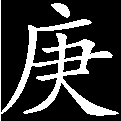
\includegraphics[width=3mm]{../Images/00004}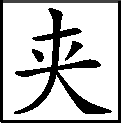
\includegraphics[width=3mm]{../Images/00012}\footnotesize \kaishu 看他用智之处。}只穿着一件松花绫子夹袄,袄内露出血点般大红裤子来。秋纹见这条红裤是晴雯手内针线,因叹道:``这条裤子以后收了罢,真是物件在人去了。''麝月忙也笑道:``这是晴雯的针线。''又叹道:``真真物在人亡了!''秋纹将麝月拉了一把,笑道:``这裤子配着松花色袄儿、石青靴子,越显出这靛青的头,雪白的脸来了。''宝玉在前只装听不见,又走了两步,便止步道:``我要走一走,这怎么好?''麝月道:``大白日里,还怕什么?还怕丢了你不成!''因命两个小丫头跟着,``我们送了这些东西去再来。''宝玉道:``好姐姐,等一等我再去。''麝月道:``我们去了就来。两个人手里都有东西,倒像摆执事的,一个捧着文房四宝,一个捧着冠袍带履,成个什么样子。''宝玉听见,正中心怀,便让他两个去了。

他便带了两个小丫头到一石后,也不怎么样,只问他二人道:``自我去了,你袭人姐姐打发人瞧晴雯姐姐去了不曾?''这一个答道:``打发宋妈妈瞧去了。''宝玉道:``回来说什么?''小丫头道:``回来说晴雯姐姐直着脖子叫了一夜,今日早起就闭了眼、住了口,世事不知,也出不得一声儿,只有倒气的分儿了。''宝玉忙道:``一夜叫的是谁?''小丫头子说:``一夜叫的是娘。''宝玉拭泪道:``还叫谁?''小丫头子道:``没有听见叫别人了。''宝玉道:``你糊涂,想必没有听真。''

旁边那一个小丫头最伶俐,听宝玉如此说,便上来说:``真个他糊涂。''又向宝玉道:``不但我听得真切,我还亲自偷着看去的。''宝玉听说,忙问:``你怎么又亲自看去?''小丫头道:``我因想晴雯姐姐素日与别人不同,待我们极好。如今他虽受了委屈出去,我们不能别的法子救他,只亲去瞧瞧,也不枉素日疼我们一场。就是人知道了回了太太,打我们一顿,也是愿受的。所以我拚着挨一顿打,偷着下去瞧了一瞧。谁知他平生为人聪明,至死不变。他因想着那起俗人不可说话,所以只闭眼养神,见我去了便睁开眼,拉我的手问:`宝玉那去了?'我告诉他实情。他叹了一口气说:`不能见了。'我就说:`姐姐何不等一等他回来见一面,岂不两完心愿?'他就笑道:`你们还不知道。我不是死,如今天上少了一位花神,玉皇敕命我去司主。我如今在未正二刻到任司花,宝玉须待未正三刻才到家,只少得一刻的工夫,不能见面。世上凡该死之人阎王勾取了过去,是差些小鬼来捉人魂魄。若要迟延一时半刻,不过烧些纸钱浇些浆饭,那鬼只顾抢钱去了,该死的人就可多待些个工夫。{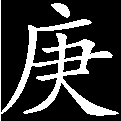
\includegraphics[width=3mm]{../Images/00004}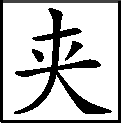
\includegraphics[width=3mm]{../Images/00012}\footnotesize \kaishu 好,奇之至!又从来皆说``阎王注定三更死,谁能留人至五更''之语,今忽借此小女儿一篇无稽之谈,反成无人敢翻之案。且又寓意调侃,骂尽世态。岂非``{[}奇{]}之至''文章耶?寄语观者:至此{(一)}{[}不{]}浮一大白者,以后不必看书也。}我这如今是有天上的神仙来召请,岂可捱得时刻!'我听了这话,竟不大信,及进来到房里留神看时辰表时,果然是未正二刻他咽了气,正三刻上就有人来叫我们,说你来了。这时候倒都对合。''

宝玉忙道:``你不识字看书,所以不知道。这原是有的,不但花有一个神,一样花有一位神之外还有总花神。但他不知是作总花神去了,还是单管一样花的神?''这丫头听了,一时诌不出来。恰好这是八月时节,园中池上芙蓉正开。这丫头便见景生情,忙答道:``我也曾问他是管什么花的神,告诉我们日后也好供养的。他说:`天机不可泄漏。你既这样虔诚,我只告诉你,你只可告诉宝玉一人。除他之外若泄了天机,五雷就来轰顶的。'他就告诉我说,他就是专管这芙蓉花的。''宝玉听了这话,不但不为怪,亦且去悲而生喜,乃指芙蓉笑道:``此花也须得这样一个人去司掌。我就料定他那样的人必有一番事业做的。虽然超出苦海,从此不能相见,也免不得伤感思念。''因又想:``虽然临终未见,如今且去灵前一拜,也算尽这五六年的情常。''

想毕忙至房中,又另穿戴了,只说去看黛玉,遂一人出园来,往前次之处去,意为停柩在内。谁知他哥嫂见他一咽气便回了进去,希图早些得几两发送例银。王夫人闻知,便命赏了十两烧埋银子。又命:``即刻送到外头焚化了罢。女儿痨死的,断不可留!''他哥嫂听了这话,一面得银,一面就雇了人来入殓,抬往城外化人场上去了。剩的衣履簪环,约有三四百金之数,他兄嫂自收了为后日之计。二人将门锁上,一同送殡去未回。宝玉走来扑了个空。{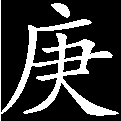
\includegraphics[width=3mm]{../Images/00004}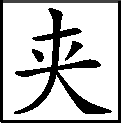
\includegraphics[width=3mm]{../Images/00012}\footnotesize \kaishu 收拾晴雯,{(故)}{[}固{]}为红颜一哭,然亦大令人不堪。◇上云王夫人怕女儿痨不祥,今则忽从宝玉心中道其苦。◇又非模拟出,是己悒郁其词,其母子之心中体贴眷爱之情,曲委已尽。}

宝玉自立了半天,别无法儿,只得复身进入园中。待回至房中,甚觉无味,因乃顺路来找黛玉。偏黛玉不在房中,问其何往,丫鬟们回说:``往宝姑娘那里去了。''宝玉又至蘅芜苑中,只见寂静无人,房内搬的空空落落的,不觉吃一大惊。忽见个老婆子走来,宝玉忙问这是什么原故。老婆子道:``宝姑娘出去了。这里交我们看着,还没有搬清楚。我们帮着送了些东西去,这也就完了。你老人家请出去罢,让我们扫扫灰尘。也好,从此你老人家省跑这一处的腿子了。''宝玉听了,怔了半天,因看着那院中的香藤异蔓,仍是翠翠青青,忽比昨日好似改作凄凉了一般,更又添了伤感。默默出来,又见门外的一条翠樾埭上也半日无人来往,不似当日各处房中丫鬟不约而来者络绎不绝。又俯身看\elegantpar{那埭下之水,仍是溶溶脉脉的流将过去。心下因想:``天地间竟有这样无情的事!}{世事总如此}''悲感一番,忽又想到去了司棋、入画、芳官等五个;死了晴雯;今又去了宝钗等一处;迎春虽尚未去,然连日也不见回来。且接连有媒人来求亲,大约园中之人不久都要散的了。纵生烦恼,也无济于事。不如还是找黛玉去相伴一日,回来还是和袭人厮混,只这两三个人,只怕还是同死同归的。想毕,仍往潇湘馆来,偏黛玉尚未回来。宝玉想亦当出去候送才是,无奈不忍悲感,还是不去的是,遂又垂头丧气的回来。

正在不知所以之际,忽见王夫人的丫头进来找他说:``老爷回来了,找你呢,又得了好题目来了。快走,快走。''宝玉听了,只得跟了出来。到王夫人房中,他父亲已出去了。王夫人命人送宝玉至书房中。

彼时贾政正与众幕友们谈论寻秋之胜,又说:``快散时忽然谈及一事,最是千古佳谈,`风流隽逸,忠义慷慨'八字皆备,倒是个好题目,大家要作一首挽词。''众幕宾听了,都忙请教系何等妙事。贾政乃道:``当日曾有一位王,封曰恒王,出镇青州。这恒王最喜女色,且公馀好武,因选了许多美女,日习武事。每公馀辄开宴连日,令众美女习战斗攻拔之事。其姬中有姓林行四者,姿色既冠,且武艺更精,皆呼为林四娘。恒王最得意,遂超拔林四娘统辖诸姬,又呼为`姽婳将军'。''众清客都称``妙极神奇。竟以`姽婳'下加`将军'二字,反更觉妩媚风流,真绝世奇文也。想这恒王也是千古第一风流人物了。''贾政笑道:``这话自然是如此,但更有可奇可叹之事。''众清客都愕然惊问道:``不知底下有何奇事?''贾政道:``谁知次年便有`黄巾'`赤眉'一干流贼馀党复又乌合,抢掠山左一带。{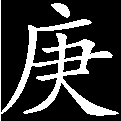
\includegraphics[width=3mm]{../Images/00004}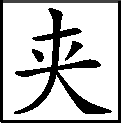
\includegraphics[width=3mm]{../Images/00012}\footnotesize \kaishu 妙!``赤眉''``黄巾''两时之事,今合而为一,盖云不过是此等众类,非特历历指明某赤某黄。若云不合两用便呆矣。此书全是如此,为混人也。}恒王意为犬羊之恶,不足大举,因轻骑前剿。不意贼众颇有诡谲智术,两战不胜,恒王遂为众贼所戮。于是青州城内文武官员,各各皆谓:`王尚不胜,你我何为!'遂将有献城之举。林四娘得闻凶报,遂集聚众女将,发令说道:`你我皆向蒙王恩,戴天履地,不能报其万一。今王既殒身国事,我意亦当殒身于王。尔等有愿随者,即时同我前往;有不愿者,亦早各散。'众女将听他这样,都一齐说愿意。于是林四娘带领众人连夜出城,直杀至贼营里头。众贼不防,也被斩戮了几员首贼。然后大家见是不过几个女人,料不能济事,遂回戈倒兵,奋力一阵,把林四娘等一个不曾留下,倒作成了这林四娘的一片忠义之志。后来报至中都,自天子以至百官,无不惊骇道奇。其后朝中自然又有人去剿灭,天兵一到,化为乌有,不必深论。只就林四娘一节,众位听了,可羡不可羡呢?''众幕友都叹道:``实在可羡可奇,实是个妙题,原该大家挽一挽才是。''说着,早有人取了笔砚,按贾政口中之言稍加改易了几个字,便成了一篇短序,递与贾政看了。贾政道:``不过如此。他们那里已有原序。昨日因又奉恩旨,着察核前代以来应加褒奖而遗落未经请奏各项人等,无论僧尼乞丐与女妇人等,有一事可嘉,即行汇送履历至礼部备请恩奖。所以他这原序也送往礼部去了。大家听见这新闻,所以都要作一首《姽婳词》,以志其忠义。''众人听了,都又笑道:``这原该如此。只是更可羡者,本朝皆系千古未有之旷典隆恩,实历代所不及处,可谓`圣朝无阙事',唐朝人预先竟说了,竟应在本朝。如今年代方不虚此一句。''贾政点头道:``正是。''

说话间,贾环叔侄亦到。贾政命他们看了题目。他两个虽能诗,较腹中之虚实虽也去宝玉不远,但第一件他两个终是别路,若论举业一道,似高过宝玉,若论杂学,则远不能及;第二件他二人才思滞钝,不及宝玉空灵娟逸,每作诗亦如八股之法,未免拘板庸涩。那宝玉虽不算是个读书人,然亏他天性聪敏,且素喜好些杂书,他自为古人中也有杜撰的,也有误失之处,拘较不得许多;若只管怕前怕后起来,纵堆砌成一篇,也觉得甚无趣味。因心里怀着这个念头,每见一题,不拘难易,他便毫无费力之处,就如世上的流嘴滑舌之人,无风作有,信着伶口俐舌,长篇大论,胡扳乱扯,敷演出一篇话来。虽无稽考,却都说得四座春风。虽有正言厉语之人,亦不得压倒这一种风流去。近日贾政年迈,名利大灰,然起初天性也是个诗酒放诞之人,因在子侄辈中,少不得规以正路。近见宝玉虽不读书,竟颇能解此,细评起来,也还不算十分玷辱了祖宗。就思及祖宗们,各各亦皆如此,虽有深精举业的,也不曾发迹过一个,看来此亦贾门之数。况母亲溺爱,遂也不强以举业逼他了。所以近日是这等待他。又要环兰二人举业之馀,怎得亦同宝玉才好,所以每欲作诗,必将三人一齐唤来对作。{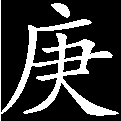
\includegraphics[width=3mm]{../Images/00004}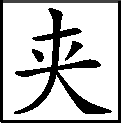
\includegraphics[width=3mm]{../Images/00012}\footnotesize \kaishu 妙!世事皆不可无足餍,只有``读书''二字是万不可足餍的。父母之心可不甚哉!近之父母只怕儿子不能名利,岂不可叹乎?}

闲言少述。且说贾政又命他三人各吊一首,谁先成者赏,佳者额外加赏。贾环贾兰二人近日当着多人皆作过几首了,胆量愈壮,今看了题,遂自去思索。一时,贾兰先有了。贾环生恐落后也就有了。二人皆已录出,宝玉\elegantpar{尚出神}{该当出神}。{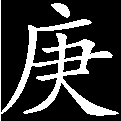
\includegraphics[width=3mm]{../Images/00004}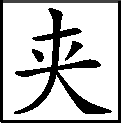
\includegraphics[width=3mm]{../Images/00012}\footnotesize \kaishu 妙,偏写出钝态来。}贾政与众人且看他二人的二首。贾兰的是一首七言绝,写道是:

姽婳将军林四娘,玉为肌骨铁为肠,

捐躯自报恒王后,此日青州土亦香。

众幕宾看了,便皆大赞:``小哥儿十三岁的人就如此,可知家学渊源,真不诬矣。''贾政笑道:``稚子口角,也还难为他。''又看贾环的,是首五言律,写道是:

红粉不知愁,将军意未休。

掩啼离绣幕,抱恨出青州。

自谓酬王德,讵能复寇仇。

谁题忠义墓,千古独风流。

众人道:``更佳。倒是大几岁年纪,立意又自不同。''贾政道:``还不甚大错,终不恳切。''众人道:``这就罢了。三爷才大不多两岁,在未冠之时如此,用了工夫,再过几年,怕不是大阮小阮了。''贾政笑道:``过奖了。只是不肯读书过失。''

因又问宝玉怎样。众人道:``二爷细心镂刻,定又是风流悲感,不同此等的了。''宝玉笑道:``这个题目似不称近体,须得古体,或歌或行,长篇一首,方能恳切。''众人听了,都立身点头拍手道:``我说他立意不同!每一题到手,必先度其体格宜与不宜,这便是老手妙法。就如裁衣一般,未下剪时,须度其身量。这题目名曰《姽婳词》,且既有了序,此必是长篇歌行方合体的。或拟白乐天《长恨歌》,\href{../Text/part0082_split_000.html\#lnkback_1_a}{\textsuperscript{①}}或拟咏古词,半叙半咏,流利飘逸,始能尽妙。''贾政听说,也合了主意,遂自提笔向纸上要写,又向宝玉笑道:``如此,你念我写。若不好了,我捶你那肉。谁许你先大言不惭了!''宝玉只得念了一句,道是:

恒王好武兼好色,

贾政写了看时,摇头道:``粗鄙。''一幕宾道:``要这样方古,究竟不粗。且看他底下的。''贾政道:``姑存之。''宝玉又道:

遂教美女习骑射。

秾歌艳舞不成欢,列阵挽戈为自得。

贾政写出,众人都道:``只这第三句便古朴老健,极妙。这四句平叙出,也最得体。''贾政道:``休谬加奖誉,且看转的如何。''宝玉念道:

眼前不见尘沙起,将军俏影红灯里。

众人听了这两句,便都叫:``妙!好个`不见尘沙起'!又承了一句`俏影红灯里',用字用句,皆入神化了。''宝玉道:

叱吒时闻口舌香,霜矛雪剑娇难举。

众人听了,便拍手笑道:``益发画出来了。当日敢是宝公也在座,见其娇且闻其香否?不然,何体贴至此。''宝玉笑道:``闺阁习武,任其勇悍,怎似男人。{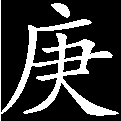
\includegraphics[width=3mm]{../Images/00004}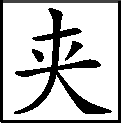
\includegraphics[width=3mm]{../Images/00012}\footnotesize \kaishu 贾老在座,故不便出``浊物''二字,妙甚细甚!}不待问而可知娇怯之形的了。''贾政道:``还不快续,这又有你说嘴的了。''宝玉只得又想了一想,念道:

丁香结子芙蓉绦,

众人都道:``转`绦',萧韵,更妙,这才流利飘荡。而且这一句也绮靡秀媚的妙。''贾政写了,看道:``这一句不好。已写过`口舌香'`娇难举',何必又如此。这是力量不加,故又用这些堆砌货来搪塞。''宝玉笑道:``长歌也须得要些词藻点缀点缀,不然便觉萧索。''贾政道:``你只顾用这些,但这一句底下如何能转至武事?若再多说两句,岂不蛇足了。''宝玉道:``如此,底下一句转煞住,想亦可矣。''贾政冷笑道:``你有多大本领?上头说了一句大开门的散话,如今又要一句连转带煞,岂不心有馀而力不足些。''宝玉听了,垂头想了一想,说了一句道:

不系明珠系宝刀。

忙问:``这一句可还使得?''众人拍案叫绝。贾政写了,看着笑道:``且放着,再续。''宝玉道:``若使得,我便要一气下去了。若使不得,越性涂了,我再想别的意思出来,再另措词。''贾政听了,便喝道:``多话!不好了再作,便作十篇百篇,还怕辛苦了不成!''宝玉听说,只得想了一会,便念道:

战罢夜阑心力怯,脂痕粉渍污鲛鮹。

贾政道:``又一段。底下怎样?''宝玉道:

明年流寇走山东,强吞虎豹势如蜂。

众人道:``好个`走'字!便见得高低了。且通句转的也不板。''宝玉又念道:

王率天兵思剿灭,一战再战不成功。

腥风吹折陇头麦,日照旌旗虎帐空。

青山寂寂水澌澌,正是恒王战死时。

雨淋白骨血染草,月冷黄沙鬼守尸。

众人都道:``妙极,妙极!布置、叙事、词藻,无不尽美。且看如何至四娘,必另有妙转奇句。''宝玉又念道:

纷纷将士只保身,青州眼见皆灰尘,

不期忠义明闺阁,愤起恒王得意人。

众人都道:``铺叙得委婉。''贾政道:``太多了,底下只怕累赘呢。''宝玉乃又念道:

恒王得意数谁行,就死将军林四娘,

号令秦姬驱赵女,艳李秾桃临战场。

绣鞍有泪春愁重,铁甲无声夜气凉。

胜负自然难预定,誓盟生死报前王。

贼势猖獗不可敌,柳折花残实可伤,

魂依城郭家乡近,马践胭脂骨髓香。

星驰时报入京师,谁家儿女不伤悲!

天子惊慌恨失守,此时文武皆垂首。

何事文武立朝纲,不及闺中林四娘!

我为四娘长太息,歌成馀意尚旁徨。

念毕,众人都大赞不止,又都从头看了一遍。贾政笑道:``虽然说了几句,到底不大恳切。''因说:``去罢。''三人如得了赦的一般,一齐出来,各自回房。

众人皆无别话,不过至晚安歇而已。独有宝玉一心凄楚,回至园中,猛然见池上芙蓉,想起小丫鬟说晴雯作了芙蓉之神,不觉又喜欢起来,乃看着芙蓉嗟叹了一会。忽又想起死后并未到灵前一祭,如今何不在芙蓉前一祭,岂不尽了礼,比俗人去灵前祭吊又更觉别致。想毕,便欲行礼。忽又止住道:``虽如此,亦不可太草率,也须得衣冠整齐,奠仪周备,方为诚敬。''想了一想,``如今若学那世俗之奠礼,断然不可;竟也还别开生面,另立排场,风流奇异,于世无涉,方不负我二人之为人。况且古人有云:`潢污行潦,苹蘩薀藻之贱,可以羞王公,荐鬼神。'原不在物之贵贱,全在心之诚敬而已。此其一也。二则诔文挽词也须另出己见,自放手眼,亦不可蹈袭前人的套头,填写几字搪塞耳目之文,亦必须洒泪泣血,一字一咽,一句一啼,宁使文不足悲有馀,万不可尚文藻而反失悲戚。况且古人多有微词,非自我今作俑也。奈今人全惑于功名二字,尚古之风一洗皆尽,恐不合时宜,于功名有碍之故。我又不希罕那功名,不为世人观阅称赞,何必不远师楚人之《大言》、《招魂》、《离骚》、《九辩》、《枯树》、《问难》、《秋水》、《大人先生传》等法,或杂参单句,或偶成短联,或用实典,或设譬寓,随意所之,信笔而去,喜则以文为戏,悲则以言志痛,辞达意尽为止,何必若世俗之拘拘于方寸之间哉。''宝玉本是个不读书之人,再心中有了这篇歪意,怎得有好诗文作出来。他自己却任意纂著,并不为人知慕,所以大肆妄诞,竟杜撰成一篇长文,用晴雯素日所喜之冰鲛縠一幅楷字写成,名曰《芙蓉女儿诔》,前序后歌。又备了四样晴雯所喜之物,于是夜月下,命那小丫头捧至芙蓉花前。先行礼毕,将那诔文即挂于芙蓉枝上,乃泣涕念曰:{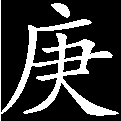
\includegraphics[width=3mm]{../Images/00004}诸君阅至此,只当一笑话看去,便可醒倦。}\href{../Text/part0082_split_000.html\#lnkback_2_a}{\textsuperscript{②}}

维太平不易之元,{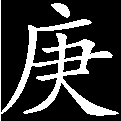
\includegraphics[width=3mm]{../Images/00004}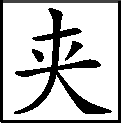
\includegraphics[width=3mm]{../Images/00012}\footnotesize \kaishu 年便奇。}蓉桂竞芳之月,{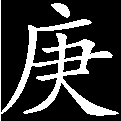
\includegraphics[width=3mm]{../Images/00004}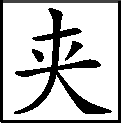
\includegraphics[width=3mm]{../Images/00012}\footnotesize \kaishu 是八月。}无可奈何之日,{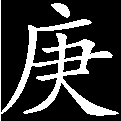
\includegraphics[width=3mm]{../Images/00004}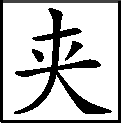
\includegraphics[width=3mm]{../Images/00012}\footnotesize \kaishu 日更奇。细思日何难于直说某某,今偏用如此说,则可知矣。}怡红院浊玉,{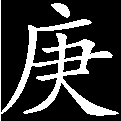
\includegraphics[width=3mm]{../Images/00004}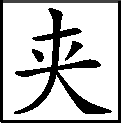
\includegraphics[width=3mm]{../Images/00012}\footnotesize \kaishu 自谦的更奇。盖常以``浊''字评天下之男子,竟自谓,所谓``以责人之心责己''矣。}谨以群花之蕊,{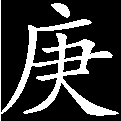
\includegraphics[width=3mm]{../Images/00004}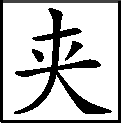
\includegraphics[width=3mm]{../Images/00012}\footnotesize \kaishu 奇香。}冰鲛之縠,{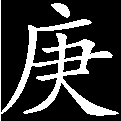
\includegraphics[width=3mm]{../Images/00004}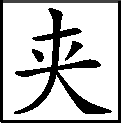
\includegraphics[width=3mm]{../Images/00012}\footnotesize \kaishu 奇帛。}沁芳之泉,{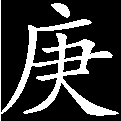
\includegraphics[width=3mm]{../Images/00004}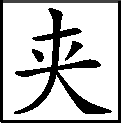
\includegraphics[width=3mm]{../Images/00012}\footnotesize \kaishu 奇奠。}枫露之茗:{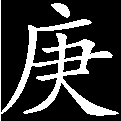
\includegraphics[width=3mm]{../Images/00004}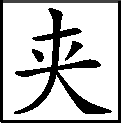
\includegraphics[width=3mm]{../Images/00012}\footnotesize \kaishu 奇茗。}四者虽微,聊以达诚申信,乃致祭于白帝宫中抚司秋艳芙蓉女儿{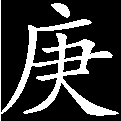
\includegraphics[width=3mm]{../Images/00004}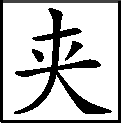
\includegraphics[width=3mm]{../Images/00012}\footnotesize \kaishu 奇称。}之前曰:

窃思女儿自临浊世,{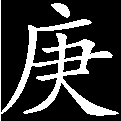
\includegraphics[width=3mm]{../Images/00004}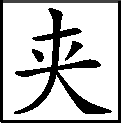
\includegraphics[width=3mm]{../Images/00012}\footnotesize \kaishu 世不浊,因物所混而浊也,前后便有照应。◇``女儿''称妙!盖思普天下之称断不能有如此二字之清洁者。亦是宝玉之真心。}迄今凡十有六载。{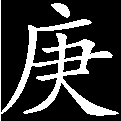
\includegraphics[width=3mm]{../Images/00004}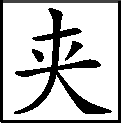
\includegraphics[width=3mm]{../Images/00012}\footnotesize \kaishu 方十六岁而夭,亦伤矣。}其先之乡籍姓氏,湮沦而莫能考者久矣。{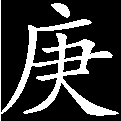
\includegraphics[width=3mm]{../Images/00004}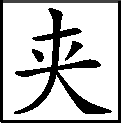
\includegraphics[width=3mm]{../Images/00012}\footnotesize \kaishu 忽又有此文。不可{(后)}{[}考何{]}来,亦可伤矣。}而玉得于衾枕栉沐之间,栖息宴游之夕,亲昵狎亵,相与共处者,仅五年八月有奇。{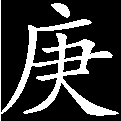
\includegraphics[width=3mm]{../Images/00004}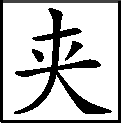
\includegraphics[width=3mm]{../Images/00012}\footnotesize \kaishu 相共不足六载,一旦夭别,岂不可伤!}忆女儿曩生之昔,其为质则金玉不足喻其贵,其为性则冰雪不足喻其洁,其为神则星日不足喻其精,其为貌则花月不足喻其色。姊妹悉慕媖娴,妪媪咸仰惠德。孰料鸠鸩恶其高,鹰鸷翻遭罦罬;{{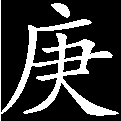
\includegraphics[width=3mm]{../Images/00004}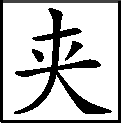
\includegraphics[width=3mm]{../Images/00012}\footnotesize \kaishu 《离骚》:``鸷鸟之不群兮。''又:``吾令鸩为媒兮,鸩告余以不好。雄鸠之鸣逝兮,余恶其轻佻。''注:鸷特立不群,故不群,故不于。鸩羽毒杀人。鸠多声,有如人之多言不实。}罦罬{,音孚拙,翻毕网。《诗经》:``雉离于}罦{。''《尔雅》:``}罬{谓之}罦{。''}}薋葹妒其臭,茝兰竟被芟鉏!{{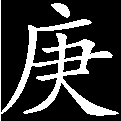
\includegraphics[width=3mm]{../Images/00004}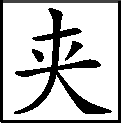
\includegraphics[width=3mm]{../Images/00012}\footnotesize \kaishu 《离骚》:}薋{、}葹{皆恶草,以辨邪佞。}茝{兰芳草,以别君子。}}花原自怯,岂奈狂飙;柳本多愁,何禁骤雨。偶遭蛊虿之谗,遂抱膏肓之疚。故尔樱唇红褪,韵吐呻吟;杏脸香枯,色陈顑颔。{{\includegraphics[width=3mm]{../Images/00004}\includegraphics[width=3mm]{../Images/00012}\footnotesize \kaishu 《离骚》:``长}顑{颔亦何伤。''面黄色。}}诼谣謑诟,出自屏帏;荆棘蓬榛,蔓延户牖。岂招尤则替,实攘诟而终。{\includegraphics[width=3mm]{../Images/00004}\includegraphics[width=3mm]{../Images/00012}\footnotesize \kaishu 《离骚》:``朝谇夕替。''废也。``忍尤而攘诟。''诟同攘,取也。}既忳幽沉于不尽,复含罔屈于无穷。高标见嫉,闺帏恨比长沙;{\includegraphics[width=3mm]{../Images/00004}\includegraphics[width=3mm]{../Images/00012}\footnotesize \kaishu 汲黯辈嫉贾谊之才,谪贬长沙。}直烈遭危,巾帼惨于羽野。{{\includegraphics[width=3mm]{../Images/00004}\includegraphics[width=3mm]{../Images/00012}\footnotesize \kaishu 鲧刚直自命,舜殛于羽山。《离骚》曰:``鲧}婞{直以亡身兮,终然}殀{乎羽之野。''}}自蓄辛酸,谁怜夭折!仙云既散,芳趾难寻。洲迷聚窟,何来却死之香?海失灵槎,不获回生之药。眉黛烟青,昨犹我画;指环玉冷,今倩谁温?鼎炉之剩药犹存,襟泪之馀痕尚渍。镜分鸾别,愁开麝月之奁;梳化龙飞,哀折檀云之齿。委金钿于草莽,拾翠?于尘埃。楼空鳷鹊,徒悬七夕之针;带断鸳鸯,谁续五丝之缕?况乃金天属节,白帝司时,孤衾有梦,空室无人。桐阶月暗,芳魂与倩影同销;蓉帐香残,娇喘共细言皆绝。连天衰草,岂独蒹葭;匝地悲声,无非蟋蟀。露苔晚砌,穿帘不度寒砧;雨荔秋垣,隔院希闻怨笛。芳名未泯,檐前鹦鹉犹呼;艳质将亡,槛外海棠预老。{\includegraphics[width=3mm]{../Images/00004}\includegraphics[width=3mm]{../Images/00012}\footnotesize \kaishu 恰极!}\elegantpar{捉迷屏后,莲瓣无声;}{晴雯缠脚}{\includegraphics[width=3mm]{../Images/00004}\includegraphics[width=3mm]{../Images/00012}\footnotesize \kaishu 元微之诗:``小楼深迷藏。''}斗草庭前,兰芽枉待。抛残绣线,银笺彩缕谁裁?折断冰丝,金斗御香未熨。昨承严命,既趋车而远陟芳园;今犯慈威,复拄杖而近抛孤匶。{\includegraphics[width=3mm]{../Images/00004}\includegraphics[width=3mm]{../Images/00012}\footnotesize \kaishu 柩本字。}及闻槥棺被燹,惭违共穴之盟;石椁成灾,愧迨同灰之诮。{\includegraphics[width=3mm]{../Images/00004}\includegraphics[width=3mm]{../Images/00012}\footnotesize \kaishu 唐诗云:``光开石棺,木可为棺。''晋杨公回诗云:``生为并身杨,死作同棺灰。''}尔乃西风古寺,淹滞青磷;落日荒丘,零星白骨。楸榆飒飒,蓬艾萧萧。隔雾圹以啼猿,绕烟塍而泣鬼。自为红绡帐里,公子情深;始信黄土垄中,女儿命薄!汝南泪血,斑斑洒向西风;梓泽馀衷,默默诉凭冷月。呜呼!固鬼蜮之为灾,岂神灵而亦妒。箝诐奴之口,讨岂从宽;剖悍妇之心,忿犹未释!{{\includegraphics[width=3mm]{../Images/00004}\includegraphics[width=3mm]{../Images/00012}\footnotesize \kaishu 《庄子》:``箝杨墨之口。''《孟子》谓:``}诐{辞知其所蔽。''}}在君之尘缘虽浅,然玉之鄙意岂终。因蓄惓惓之思,不禁谆谆之问。始知上帝垂旌,花宫待诏,生侪兰蕙,死辖芙蓉。听小婢之言,似涉无稽;以浊玉之思,则深为有据。何也?昔叶法善摄魂以撰碑,李长吉被诏而为记,事虽殊,其理则一也。故相物以配才,苟非其人,恶乃滥乎?始信上帝委托权衡,可谓至洽至协,庶不负其所秉赋也。因希其不昧之灵,或陟降于兹;特不揣鄙俗之词,有污慧听。乃歌而招之曰:

天何如是之苍苍兮,乘玉虬以游乎穹窿耶?{{\includegraphics[width=3mm]{../Images/00004}\includegraphics[width=3mm]{../Images/00012}\footnotesize \kaishu 《楚辞》:``驷玉虬以乘}鹥{兮。''}}

地何如是之茫茫兮,驾瑶象以降乎泉壤耶?{\includegraphics[width=3mm]{../Images/00004}\includegraphics[width=3mm]{../Images/00012}\footnotesize \kaishu 《楚辞》:``杂瑶象以为车。''}

望伞盖之陆离兮,抑箕尾之光耶?

列羽葆而为前导兮,卫危虚于旁耶?

驱丰隆以为比从兮,望舒月以离耶?{\includegraphics[width=3mm]{../Images/00004}\includegraphics[width=3mm]{../Images/00012}\footnotesize \kaishu 危、虚二星为卫护星。丰隆,雷师。望舒,月御也。}

听车轨而伊轧兮,御鸾鷖以征耶?

闻馥郁而薆然兮,纫蘅杜以为纕耶?

炫裙裾之烁烁兮,镂明月以为珰耶?

籍葳蕤而成坛畤兮,檠莲焰以烛兰膏耶?

文瓟匏以为觯斝兮,漉醽醁以浮桂醑耶?

瞻云气而凝盼兮,仿佛有所觇耶?

俯窈窕而属耳兮,恍惚有所闻耶?

期汗漫而无夭阏兮,忍捐弃余于尘埃耶?{\includegraphics[width=3mm]{../Images/00004}\includegraphics[width=3mm]{../Images/00012}\footnotesize \kaishu 《逍遥游》:夭阏,止也。}

倩风廉之为余驱车兮,冀联辔而携归耶?

余中心为之慨然兮,{\includegraphics[width=3mm]{../Images/00004}\includegraphics[width=3mm]{../Images/00012}\footnotesize \kaishu 《庄子·至乐篇》:``我独何能无慨然?''}徒噭噭而何为耶?{{\includegraphics[width=3mm]{../Images/00004}\includegraphics[width=3mm]{../Images/00012}\footnotesize \kaishu 《庄子》:``}噭噭{然随而哭之。''}}

君偃然而长寝兮,岂天运之变于斯耶?{\includegraphics[width=3mm]{../Images/00004}\includegraphics[width=3mm]{../Images/00012}\footnotesize \kaishu 《庄子》:``偃然寝于巨室'',谓人死也。◇又``变而有气,气变而有形,形变而有生,今又变而之死,是相与为春秋冬夏四时行也。''◇《天道篇》:``其死也物化。''}

既窀穸且安稳兮,反其真而复奚化耶?{\includegraphics[width=3mm]{../Images/00004}\includegraphics[width=3mm]{../Images/00012}\footnotesize \kaishu 窀音肫。《左传》:``窀穸之事'',墓穴幽堂也。左贵嫔《杨后诔》:``早即窀穸。''《庄子·大宗师》:``而已反其真。''注:以死为真。}

余犹桎梏而悬附兮,灵格余以嗟来耶?{\includegraphics[width=3mm]{../Images/00004}\includegraphics[width=3mm]{../Images/00012}\footnotesize \kaishu 《庄子·大宗师》:桎梏之名。◇``彼以生为悬疣附赘,以死为决疣溃痈。''◇``嗟来桑户乎!嗟来桑户乎!''注:桑户,人名。孟子反、琴张二人,招其魂而语之也。◇``方将不化,恶知已化哉!''言人死犹如化去。《法华经》云:``法华道师多殊方便,于险道中化一城,疲极之众,入城皆生已度想,安稳想。''}

来兮止兮,君其来耶!

若夫鸿蒙而居,寂静以处,虽临于兹,余亦莫睹。搴烟萝而为步幛,列枪蒲而森行伍。警柳眼之贪眠,释莲心之味苦。素女约于桂岩,宓妃迎于兰渚。弄玉吹笙,寒簧击敔。征嵩岳之妃,启骊山之姥。龟呈洛浦之灵,兽作咸池之舞。潜赤水兮龙吟,集珠林兮凤翥。爰格爰诚,匪簠匪筥。发轫乎霞城,返旌乎玄圃。既显微而若通,复氤氲而倏阻。离合兮烟云,空蒙兮雾雨。尘霾敛兮星高,溪山丽兮月午。何心意之忡忡,若寤寐之栩栩。余乃欷歔怅望,泣涕旁徨。人语兮寂历,天籁兮筼筜。鸟惊散而飞,鱼唼喋以响。志哀兮是祷,成礼兮期祥。

呜呼哀哉!尚飨!

读毕,遂焚帛奠茗,犹依依不舍。小鬟催至再四,方才回身。忽听山石之后有一人笑道:``且请留步。''二人听了,不免一惊。那小鬟回头一看,却是个人影从芙蓉花中走出来,他便大叫:``不好,有鬼。晴雯真来显魂了!''唬得宝玉也忙看时,------且听下回分解。

{\includegraphics[width=3mm]{../Images/00005}\kaishu 总评:前文入一院,必叙一番养竹种花,为诸婆争利渲染。此文入一院,必叙一番树枯香老,为亲眷凋零凄楚。字字实境,字字奇情,令我把玩不释。}

{\kaishu 《姽婳词》一段,与前后文似断似连,如罗浮二山,烟雨为连合,时有精气来往。}

% {\href{../Text/part0082_split_000.html\#navto_1_a}{①}甲辰本此处多``或拟温八叉《击瓯歌》,或拟李长吉《会稽歌》,''两句。}

% {\href{../Text/part0082_split_000.html\#navto_2_a}{②}按:``诸君阅至此,只当一笑话看去,便可醒倦。''此评原误入正文。}
